% B.Tech Project II (EC4201) report -- group project.
% Format follows the department's Major Project Report (A4, 1.5 spacing, CHAPTER N headings).
% Build:  cd docs/report && tectonic main.tex      (or pdfLaTeX / XeLaTeX on Overleaf)
\documentclass[12pt,a4paper]{report}

% Page setup
\usepackage[a4paper,margin=1in]{geometry}
\usepackage{setspace}

% Graphics & formatting
\usepackage{graphicx}
\graphicspath{{figures/}}
\usepackage{titlesec}
\usepackage{tocloft}
\usepackage{subcaption}

% Math
\usepackage{amsmath,amssymb}

% Tables
\usepackage{longtable}
\usepackage{array}
\usepackage{booktabs}
\usepackage{multirow}
\usepackage{tabularx}

% Caption & floats
\usepackage{caption}
\usepackage{float}

% Lists, diagrams
\usepackage{enumitem}
\usepackage{tikz}
\usetikzlibrary{arrows.meta,positioning,shapes.geometric,calc,fit}
\usepackage{pgfplots}
\pgfplotsset{compat=1.17}

% Header/Footer
\usepackage{fancyhdr}

% Code Listings
\usepackage{listings}
\usepackage{xcolor}

\definecolor{codegreen}{rgb}{0,0.6,0}
\definecolor{codegray}{rgb}{0.45,0.45,0.45}
\definecolor{codepurple}{rgb}{0.58,0,0.82}
\definecolor{backcolour}{rgb}{0.97,0.97,0.97}

\lstdefinestyle{codebox}{
    backgroundcolor=\color{backcolour},
    commentstyle=\color{codegreen}\itshape,
    keywordstyle=\color{blue}\bfseries,
    numberstyle=\tiny\color{codegray},
    stringstyle=\color{codepurple},
    basicstyle=\ttfamily\scriptsize,
    breakatwhitespace=false,
    breaklines=true,
    captionpos=b,
    keepspaces=true,
    numbers=left,
    numbersep=5pt,
    showspaces=false,
    showstringspaces=false,
    showtabs=false,
    tabsize=2,
    frame=single,
    rulecolor=\color{black!20}
}
\lstset{style=codebox}

% Formatting tweaks
\overfullrule=0pt
\setlength{\emergencystretch}{3em}
\onehalfspacing
\setlength{\parindent}{0pt}
\setlength{\parskip}{6pt}
\setlist{nosep,leftmargin=*,topsep=2pt}

% Custom column types
\newcolumntype{L}[1]{>{\raggedright\arraybackslash}p{#1}}
\newcolumntype{C}[1]{>{\centering\arraybackslash}p{#1}}

% Header/Footer setup
\pagestyle{fancy}
\fancyhf{}
\fancyfoot[C]{\thepage}
\renewcommand{\headrulewidth}{0pt}
\fancypagestyle{plain}{\fancyhf{}\fancyfoot[C]{\thepage}\renewcommand{\headrulewidth}{0pt}}

% Chapter formatting
\titleformat{\chapter}[display]
{\normalfont\bfseries\centering\Large}
{CHAPTER \thechapter}
{0.5em}
{\Large}
% Unnumbered titles (Declaration, ABSTRACT, ...): bold, centred
\titleformat{name=\chapter,numberless}[block]{\normalfont\bfseries\centering\Large}{}{0pt}{}

% Contents
\setcounter{tocdepth}{2}
\renewcommand{\bibname}{REFERENCES}

% TikZ styles
\tikzset{
  blk/.style={draw,rounded corners=3pt,align=center,minimum height=1.0cm,text width=2.4cm,font=\small,fill=#1},
  blk/.default=white,
  flow/.style={draw,rounded corners=3pt,align=center,text width=4.6cm,minimum height=0.8cm,font=\small},
  dec/.style={draw,diamond,aspect=2.2,align=center,inner sep=1pt,font=\small},
  arr/.style={-{Stealth[length=2.5mm]},thick},
}

% Report details
\newcommand{\reporttitle}{Sign Language to Smart-Glasses HUD: Real-Time ISL Word Display on an ESP32-C3 OLED Head-Up Display}

% Hyperref (MUST BE LAST)
\usepackage[hidelinks,plainpages=false,pdfpagelabels]{hyperref}

\begin{document}

% ═══════════════════════════════════════════════════════════════
%  TITLE PAGE
% ═══════════════════════════════════════════════════════════════
\begin{titlepage}
\singlespacing
\centering
\vspace*{0.2cm}
{\LARGE\bfseries Sign Language to Smart-Glasses HUD:\\[4pt] Real-Time ISL Word Display on an\\[4pt] ESP32-C3 OLED Head-Up Display\par}

\vspace{0.7cm}
{\large A report submitted in partial fulfillment of the requirements\\
for the award of the degree of\\
\textbf{Bachelor of Technology}\\
in\\
\textbf{Electronics and Communication Engineering}\par}

\vspace{0.7cm}
{\large Submitted By\par}
\vspace{0.2cm}
{\large\bfseries AYUSH VERMA\par}
{\large Roll No: \textbf{230102017}\par}
\vspace{0.2cm}
{\large\bfseries CHARAN TEJ\par}
{\large Roll No: \textbf{230104002}\par}
\vspace{0.2cm}
{\large\bfseries 7th Semester\par}

\vspace{0.5cm}
{\large Supervised By\par}
\vspace{0.2cm}
{\Large\bfseries Dr. B. Somaraju\par}
{\small Assistant Professor, Department of ECE\par}

\vfill

\includegraphics[width=3cm]{iiitm_logo.png}\par
\vspace{0.5cm}
{\scshape Department of Electronics and Communication Engineering\\[3pt]
Indian Institute of Information Technology Senapati, Manipur\\[3pt]
November, 2026\par}
\end{titlepage}
\onehalfspacing

\pagenumbering{roman}

% ═══════════════════════════════════════════════════════════════
%  DECLARATION
% ═══════════════════════════════════════════════════════════════
\chapter*{Declaration}
\addcontentsline{toc}{chapter}{Declaration}

In this submission, we have expressed our ideas in our own words, and we have adequately cited and referenced any ideas or words that were taken from another source. We also declare that we adhere to all principles of academic honesty and integrity and that we have not misrepresented or falsified any ideas, data, facts, or sources in this submission. If any violation of the above is made, we understand that the institute may take disciplinary action. Such a violation may also engender disciplinary action from the sources which were not properly cited or permission not taken when needed.

\vspace{2cm}
\noindent
\begin{minipage}[t]{0.48\textwidth}
\raggedright
\textbf{Ayush Verma}\\
Roll No: 230102017\\
Department of ECE\\
IIIT Senapati, Manipur
\end{minipage}\hfill
\begin{minipage}[t]{0.48\textwidth}
\raggedleft
\textbf{Charan Tej}\\
Roll No: 230104002\\
Department of ECE\\
IIIT Senapati, Manipur
\end{minipage}

\vspace{1.5cm}
\noindent\textbf{DATE:} \underline{\hspace{4cm}}\\
\textbf{PLACE:} Senapati, Manipur

% ═══════════════════════════════════════════════════════════════
%  CERTIFICATE
% ═══════════════════════════════════════════════════════════════
\clearpage
\phantomsection
\addcontentsline{toc}{chapter}{Certificate}
\thispagestyle{plain}
\noindent
\begin{minipage}[c]{0.15\textwidth}
    \centering
    
\includegraphics[width=1.8cm]{iiitm_logo.png}
\end{minipage}%
\begin{minipage}[c]{0.8\textwidth}
    \small Department of Electronics and Communication Engineering\\
    Indian Institute of Information Technology Senapati, Manipur
\end{minipage}

\vspace{0.2cm}
\noindent\rule{\textwidth}{0.4pt}

\noindent
{\small
\begin{minipage}[t]{0.6\textwidth}
  Dr. B. Somaraju\\
  Assistant Professor, ECE, IIIT Senapati, Manipur
\end{minipage}%
\begin{minipage}[t]{0.4\textwidth}
  \raggedleft
  Email: somaraju@iiitmanipur.ac.in
\end{minipage}}

\vspace{0.8cm}
\begin{center}
{\Large\bfseries To Whom It May Concern}
\end{center}

\vspace{0.4cm}
\begin{center}
This is to certify that the project report entitled \textbf{``\reporttitle''} submitted to the Department of Electronics and Communication Engineering, Indian Institute of Information Technology Senapati, Manipur in partial fulfilment for the award of degree of \textbf{Bachelor of Technology in Electronics and Communication Engineering} is a record of bonafide work carried out by \textbf{Ayush Verma} bearing roll number \textbf{230102017} and \textbf{Charan Tej} bearing roll number \textbf{230104002} for the course \textbf{Project II (EC4201)}.
\end{center}

\vspace{1.2cm}
\begin{flushright}
\begin{minipage}{0.5\textwidth}
\centering
Signature of the Supervisor\\[6pt]
\textbf{(Dr. B. Somaraju)}
\end{minipage}
\end{flushright}

\vspace{1.2cm}
{\small
\noindent Signature of the Examiner 1 \dotfill\hspace{1em}Signature of the Examiner 2 \dotfill\\[1.2cm]
\noindent Signature of the Examiner 3 \dotfill\hspace{1em}Signature of the Examiner 4 \dotfill}

% ═══════════════════════════════════════════════════════════════
%  ABSTRACT
% ═══════════════════════════════════════════════════════════════
\chapter*{ABSTRACT}
\addcontentsline{toc}{chapter}{ABSTRACT}

People who use Indian Sign Language (ISL) are often not understood by people who do not sign. This project builds a low-cost wearable aid for the listener: a pair of glasses with a small head-up display (HUD) that shows, in real time, the words a signer is making. A laptop camera films the signer. A recognition application extracts hand and body landmarks with MediaPipe, classifies each sign with a temporal convolutional network (TCN) and builds a sentence. Each word is sent as a small JSON packet over UDP on a phone Wi-Fi hotspot.

On the glasses, an ESP32-C3 SuperMini microcontroller joins the hotspot, registers the mDNS name \texttt{glasses.local}, receives the packets on port 4210 and draws the text on a 0.96-inch SSD1306 OLED. A short word is shown large in the centre; a sentence scrolls across the screen twice. The OLED image passes through a 25\,mm lens and is reflected into the eye by a 45$^\circ$ clear acrylic sheet, so the text floats in front of the wearer. The unit runs from a 600\,mAh LiPo cell through a TP4056 protection board, and a parametric OpenSCAD enclosure that clips onto the glasses arm was designed and exported for 3D printing.

Every part was verified with a step-by-step bring-up procedure, and the link was tested end to end with typed text, simulated signing and live signing. The bench optics gave a sharp image at an OLED-to-lens distance of 22\,mm, and the measured sentence timing (14.6\,s) matched the model (14.67\,s). The work combines embedded firmware, wireless networking, optics, power electronics, mechanical CAD and machine learning in one working system.

% ═══════════════════════════════════════════════════════════════
%  ACKNOWLEDGEMENT
% ═══════════════════════════════════════════════════════════════
\chapter*{ACKNOWLEDGEMENT}
\addcontentsline{toc}{chapter}{ACKNOWLEDGEMENT}

We express our sincere gratitude to our project supervisor, Dr. B. Somaraju, for his guidance, constructive feedback and continuous encouragement throughout this project.

We also thank the Head of the Department, the Director of IIIT Manipur, and all faculty members of the Department of Electronics and Communication Engineering for the academic resources and laboratory facilities, including the bench power supply and the digital multimeter used for testing. Finally, we thank our peers and families for their constant support and motivation.

\vspace{1.5cm}
\noindent
\begin{minipage}[t]{0.48\textwidth}
\raggedright
\textbf{Ayush Verma}\\
Roll No: 230102017
\end{minipage}\hfill
\begin{minipage}[t]{0.48\textwidth}
\raggedleft
\textbf{Charan Tej}\\
Roll No: 230104002
\end{minipage}

% ═══════════════════════════════════════════════════════════════
%  CONTENTS / LISTS
% ═══════════════════════════════════════════════════════════════
\clearpage
\tableofcontents
\clearpage
\listoftables
\clearpage
\listoffigures

% ═══════════════════════════════════════════════════════════════
%  LIST OF ABBREVIATIONS
% ═══════════════════════════════════════════════════════════════
\chapter*{LIST OF ABBREVIATIONS}
\addcontentsline{toc}{chapter}{LIST OF ABBREVIATIONS}
\begin{center}
\begin{longtable}{L{3cm} L{9cm}}
\toprule
\textbf{Abbreviation} & \textbf{Expansion} \\
\midrule
\endhead
BiLSTM & Bidirectional Long Short-Term Memory \\
CAD & Computer-Aided Design \\
CC/CV & Constant Current / Constant Voltage (charging) \\
DIY & Do It Yourself \\
ECE & Electronics and Communication Engineering \\
GPIO & General-Purpose Input/Output \\
GPU & Graphics Processing Unit \\
HUD & Head-Up Display \\
I2C & Inter-Integrated Circuit (two-wire serial bus) \\
IP & Internet Protocol \\
ISL & Indian Sign Language \\
JSON & JavaScript Object Notation \\
LED & Light-Emitting Diode \\
LiPo & Lithium Polymer (battery) \\
mDNS & Multicast Domain Name System \\
ML & Machine Learning \\
OLED & Organic Light-Emitting Diode \\
PLA & Polylactic Acid (3D-printing plastic) \\
SCL & Serial Clock Line \\
SDA & Serial Data Line \\
STL & Stereolithography (3D mesh file format) \\
TCN & Temporal Convolutional Network \\
TX & Transmit \\
UDP & User Datagram Protocol \\
USB & Universal Serial Bus \\
\bottomrule
\end{longtable}
\end{center}

% ═══════════════════════════════════════════════════════════════
%  LIST OF SYMBOLS
% ═══════════════════════════════════════════════════════════════
\chapter*{LIST OF SYMBOLS}
\addcontentsline{toc}{chapter}{LIST OF SYMBOLS}
\begin{center}
\begin{longtable}{L{3cm} L{9cm}}
\toprule
\textbf{Symbol} & \textbf{Description} \\
\midrule
\endhead
$u$ & Object distance, OLED screen to lens centre (22\,mm) \\
$v$ & Image distance from the lens (mm; negative = virtual image) \\
$f$ & Focal length of the lens (estimated $\approx$ 25\,mm) \\
$m$ & Lateral magnification of the HUD image \\
$n$ & Number of characters in a displayed sentence \\
$t_{\text{pass}}$ & Time for one full scroll pass of a sentence (s) \\
$t_{\text{total}}$ & Time a sentence stays on screen, 2 passes (s) \\
$V_{5V}$ & Voltage at the ESP32-C3 5V pin (V) \\
$V_{3V3}$ & Voltage at the ESP32-C3 3V3 pin (V) \\
\bottomrule
\end{longtable}
\end{center}

\clearpage
\pagenumbering{arabic}

% ═══════════════════════════════════════════════════════════════
%  CHAPTER 1: INTRODUCTION
% ═══════════════════════════════════════════════════════════════
\chapter{INTRODUCTION}

\section{Overview}
\begin{itemize}
  \item Indian Sign Language (ISL) is the main language of the Deaf community in India.
  \item Most hearing people do not know ISL, so everyday conversations need a human interpreter.
  \item Computer vision can now track hands and body in real time on an ordinary laptop camera.
  \item Small, cheap Wi-Fi microcontrollers and OLED screens make a home-built head-up display (HUD) possible.
  \item This project combines the two: a ``caption'' for sign language that the listener sees in their glasses (Figure~\ref{fig:system}).
\end{itemize}

\begin{figure}[H]
\centering
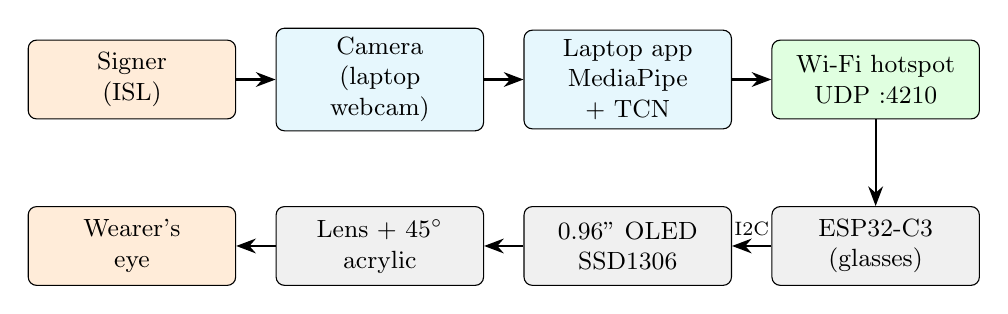
\begin{tikzpicture}[node distance=0.5cm]
  \node[blk=orange!15] (sig) {Signer\\(ISL)};
  \node[blk=cyan!10, right=of sig] (cam) {Camera\\(laptop webcam)};
  \node[blk=cyan!10, right=of cam] (lap) {Laptop app\\MediaPipe + TCN};
  \node[blk=green!12, right=of lap] (wifi) {Wi-Fi hotspot\\UDP :4210};
  \node[blk=gray!12, below=1.1cm of wifi] (esp) {ESP32-C3\\(glasses)};
  \node[blk=gray!12, left=of esp] (oled) {0.96'' OLED\\SSD1306};
  \node[blk=gray!12, left=of oled] (opt) {Lens + 45$^\circ$\\acrylic};
  \node[blk=orange!15, left=of opt] (eye) {Wearer's\\eye};
  \draw[arr] (sig) -- (cam); \draw[arr] (cam) -- (lap); \draw[arr] (lap) -- (wifi);
  \draw[arr] (wifi) -- (esp); \draw[arr] (esp) -- node[above,font=\scriptsize]{I2C} (oled);
  \draw[arr] (oled) -- (opt); \draw[arr] (opt) -- (eye);
\end{tikzpicture}
\caption{System overview: from the signer to the text in the wearer's eye}
\label{fig:system}
\end{figure}

\section{Sign Language Accessibility and Wearable HUDs}
\begin{itemize}
  \item Phone-screen captions force the listener to look away from the signer.
  \item Commercial smart glasses are expensive and closed.
  \item A low-cost DIY HUD built from hobby parts can be made and repaired by students.
  \item Earlier DIY HUD designs used weak electronics (no regulator, ESP8266-01, hard-coded IP) \cite{june}; this project fixes those.
\end{itemize}

\section{Problem Statement and Key Contributions}

\textbf{Problem statement:}
\begin{itemize}
  \item Show each recognised ISL word to a hearing person \textbf{in their field of view}, hands-free, in real time.
  \item The display unit must be \textbf{light, battery powered and wireless}, and must clip onto ordinary glasses.
  \item The text must be \textbf{sharp and readable} through simple optics (one lens and a beam combiner).
  \item The glasses and the recognizer must talk over a \textbf{simple, documented network link}.
\end{itemize}

\textbf{Key contributions:}
\begin{itemize}
  \item A step-by-step, pass/fail bring-up of every hardware part (ESP32-C3, OLED, charger, battery, switch).
  \item Wireless display firmware: mDNS discovery, UDP packets, centred words and scrolling sentences.
  \item A no-mirror HUD optics path, measured on the bench (OLED $\rightarrow$ 22\,mm $\rightarrow$ lens $\rightarrow$ 45$^\circ$ acrylic).
  \item A parametric, print-ready clip-on enclosure in OpenSCAD.
  \item A sign-recognition application (MediaPipe + TCN) that sends every word and sentence to the glasses.
  \item A written app-to-glasses interface, tested end to end.
\end{itemize}

\begin{table}[H]
\centering
\caption{Work division between the team members}
\label{tab:division}
\begin{tabularx}{\linewidth}{L{3.2cm} X}
\toprule
\textbf{Member} & \textbf{Responsibility} \\
\midrule
Ayush Verma (230102017) & Sign-recognition software: dataset preparation, MediaPipe landmarks, TCN model, training, live recognition app and UDP sender \cite{sib} \\
Charan Tej (230104002) & Hardware and firmware: ESP32-C3 + OLED display unit, LiPo power, HUD optics, 3D enclosure, glasses-side link and bring-up tests \\
Both & Shared UDP interface, integration and end-to-end testing, documentation \\
\bottomrule
\end{tabularx}
\end{table}

\section{Objectives and Scope}

\textbf{Objectives:}
\begin{enumerate}
  \item Bring up and verify every hardware part step by step.
  \item Write firmware that receives words over Wi-Fi (UDP + mDNS) and shows them clearly on the OLED.
  \item Design the HUD optics: OLED $\rightarrow$ lens $\rightarrow$ 45$^\circ$ acrylic $\rightarrow$ eye.
  \item Design a 3D-printable clip-on enclosure for the display unit.
  \item Connect the glasses to the recognizer and test the full chain end to end.
\end{enumerate}

\textbf{Scope:}
\begin{itemize}
  \item \textbf{In scope:} isolated ISL words (INCLUDE-50 \cite{include} and our own recorded words) and short sentences built from them; display unit for one eye (right); laptop as the recognition computer.
  \item \textbf{Out of scope:} continuous sentence-level sign translation; recognition running on the glasses.
  \item \textbf{Stretch goal:} an ESP32-CAM on the glasses as the camera.
\end{itemize}

\section{Report Organization}
\begin{itemize}
  \item \textbf{Chapter 2} reviews existing approaches and the theory used: microcontroller, display, network, optics and battery charging.
  \item \textbf{Chapter 3} describes the system design and implementation: electronics, firmware, optics, enclosure, recognizer and integration.
  \item \textbf{Chapter 4} presents the test results, measurements and analysis, and the challenges met with their solutions.
  \item \textbf{Chapter 5} concludes the report, lists the limitations and suggests future work.
  \item \textbf{Appendices A--D} give the wiring and parts, a firmware excerpt, the UDP interface and the bring-up sketches.
\end{itemize}

% ═══════════════════════════════════════════════════════════════
%  CHAPTER 2: LITERATURE REVIEW AND THEORETICAL BACKGROUND
% ═══════════════════════════════════════════════════════════════
\chapter{LITERATURE REVIEW AND THEORETICAL BACKGROUND}

\section{Existing Approaches and Limitations}

\begin{table}[H]
\centering
\caption{Existing ways to show sign-language output to a listener}
\label{tab:existing}
\begin{tabularx}{\linewidth}{L{3.4cm} X X}
\toprule
\textbf{Method} & \textbf{How it works} & \textbf{Limitation} \\
\midrule
Human interpreter & Person translates live & Not always available, costly \\
Phone / laptop captions & Recognised text on a screen & Listener looks away from the signer \\
Commercial smart glasses & Built-in micro display & Expensive, closed platform \\
Sensor gloves & Flex/IMU sensors on the signer's hands & Signer must wear special hardware \\
\textbf{This project} & Camera + ML on laptop, DIY HUD glasses & Needs a laptop and a hotspot \\
\bottomrule
\end{tabularx}
\end{table}

\section{Review of Related Work}
\begin{itemize}
  \item \textbf{MediaPipe} \cite{mediapipe}: real-time pipelines for hand and body landmark tracking on ordinary CPUs and GPUs; turns video into landmark sequences.
  \item \textbf{INCLUDE dataset} \cite{include}: a large ISL word dataset (263 words, 4,287 videos); its 50-word subset INCLUDE-50 is used for training.
  \item \textbf{Temporal Convolutional Networks} \cite{tcn}: 1-D dilated convolutions that match or beat recurrent networks on sequence tasks; our main recognition model is a TCN.
  \item \textbf{June\_Glasses} \cite{june}: open DIY HUD glasses; gave the optics concept (OLED, lens, beam combiner). Its electronics had no regulator and a hard-coded IP.
  \item \textbf{Adafruit SSD1306 / GFX libraries} \cite{adafruit1306,adafruitgfx}: standard Arduino drivers for the OLED, with text, bitmaps and size scaling.
  \item \textbf{OpenSCAD} \cite{openscad}: script-based CAD; every dimension is a named parameter, so the enclosure can be changed and re-exported quickly.
\end{itemize}

\section{Theoretical Background}

\subsection{ESP32-C3 Microcontroller and SSD1306 OLED}
\begin{itemize}
  \item \textbf{ESP32-C3:} 32-bit RISC-V microcontroller with Wi-Fi 802.11 b/g/n (2.4\,GHz only) and native USB \cite{esp32c3}.
  \item \textbf{SSD1306 OLED:} 128$\times$64 monochrome display driver, controlled over I2C (address 0x3C) \cite{ssd1306}.
  \item \textbf{I2C bus:} two-wire serial bus (SDA data, SCL clock) between the microcontroller and the OLED.
\end{itemize}

\subsection{Wireless Link: UDP and mDNS}
\begin{itemize}
  \item \textbf{UDP:} connectionless transport; one small datagram per word gives low delay and no connection set-up.
  \item \textbf{mDNS:} lets the laptop find the glasses by name (\texttt{glasses.local}) instead of a changing IP address.
\end{itemize}

\subsection{HUD Optics and the Thin-Lens Equation}
\begin{itemize}
  \item A convex lens placed closer to the OLED than its focal length makes a magnified \emph{virtual} image.
  \item A 45$^\circ$ clear sheet reflects the image into the eye while the world stays visible (Figure~\ref{fig:optics}).
\end{itemize}

Thin-lens equation (real-is-positive sign convention) \cite{hecht}:
\begin{equation}
\frac{1}{u} + \frac{1}{v} = \frac{1}{f}, \qquad m = -\frac{v}{u}
\label{eq:lens}
\end{equation}
where $u$ is the object (OLED) distance, $v$ the image distance and $f$ the focal length. If $u < f$, then $v < 0$: the image is virtual, upright and magnified.

\begin{figure}[H]
\centering
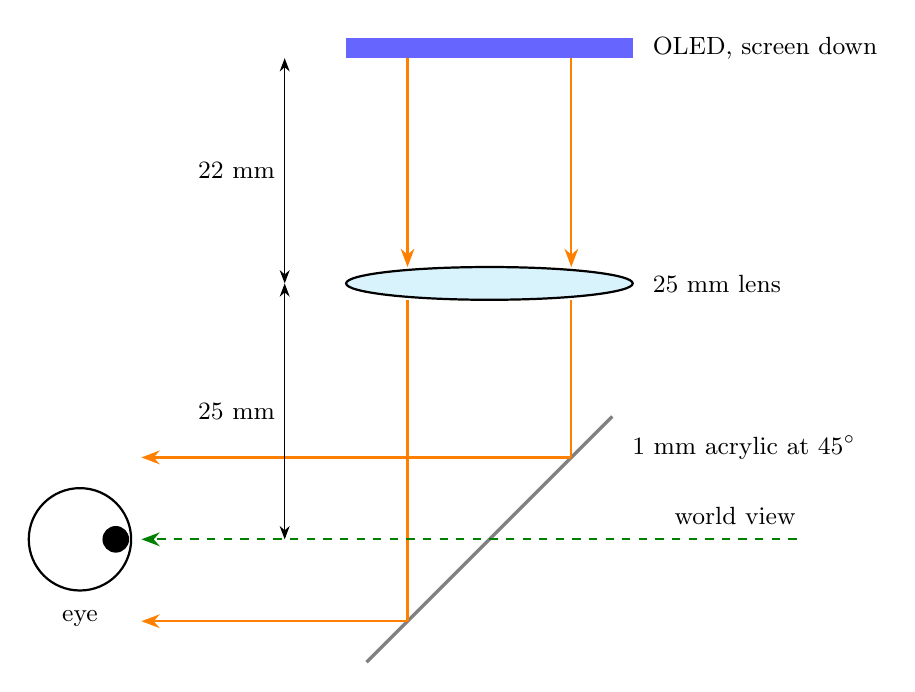
\begin{tikzpicture}[scale=0.13, every node/.style={font=\small}]
  \fill[blue!60] (-14,47) rectangle (14,49);
  \node[right] at (15,48) {OLED, screen down};
  \draw[thick,fill=cyan!15] (0,25) ellipse (14 and 1.6);
  \node[right] at (15,25) {25 mm lens};
  \draw[very thick,gray] (-12,-12) -- (12,12);
  \node[right] at (13,9) {1 mm acrylic at 45$^\circ$};
  \draw[orange,thick,-{Stealth}] (-8,47) -- (-8,26.6);
  \draw[orange,thick,-{Stealth}] (8,47) -- (8,26.6);
  \draw[orange,thick] (-8,23.4) -- (-8,-8); \draw[orange,thick] (8,23.4) -- (8,8);
  \draw[orange,thick,-{Stealth}] (-8,-8) -- (-34,-8);
  \draw[orange,thick,-{Stealth}] (8,8) -- (-34,8);
  \draw[thick] (-40,0) circle (5); \fill (-36.5,0) circle (1.3);
  \node[below] at (-40,-6) {eye};
  \draw[green!50!black,thick,dashed,-{Stealth}] (30,0) -- (-34,0);
  \node[above] at (24,0.5) {world view};
  \draw[{Stealth}-{Stealth}] (-20,47) -- node[left]{22 mm} (-20,25);
  \draw[{Stealth}-{Stealth}] (-20,25) -- node[left]{25 mm} (-20,0);
\end{tikzpicture}
\caption{HUD light path (side view): OLED $\rightarrow$ lens $\rightarrow$ 45$^\circ$ acrylic $\rightarrow$ eye}
\label{fig:optics}
\end{figure}

\subsection{Single-Cell LiPo Charging}
\begin{itemize}
  \item \textbf{TP4056:} single-cell Li-ion linear charger (CC/CV, 4.2\,V) with a protection IC \cite{tp4056}.
  \item The stock board charges at 1\,A, which is 1.7C for a 600\,mAh cell, so it is too high for our battery.
  \item Safe charging used here: a bench supply at 4.20\,V with a 0.30\,A limit, stopped when the current falls to $\le$ 0.05\,A.
\end{itemize}

\section{Identified Gap and Technical Requirements}
\begin{itemize}
  \item No low-cost, open, clip-on HUD that shows \textbf{ISL} recognition output was found.
  \item \textbf{Requirements derived for this project:}
  \begin{itemize}
    \item Wireless link with discovery by name (mDNS) and a fixed, small packet format.
    \item Readable text: large, centred words; long sentences scroll.
    \item Safe single-cell LiPo power with protection and a power switch.
    \item Adjustable focus and a mount that fits a given pair of glasses.
    \item Software-selectable mirroring (\texttt{MIRROR\_X}, \texttt{FLIP\_Y}) in case the optics flip the text.
  \end{itemize}
\end{itemize}

% ═══════════════════════════════════════════════════════════════
%  CHAPTER 3: SYSTEM DESIGN AND IMPLEMENTATION
% ═══════════════════════════════════════════════════════════════
\chapter{SYSTEM DESIGN AND IMPLEMENTATION}

\section{Design Methodology and Implementation Flow}
\begin{itemize}
  \item We followed a ``test every part first'' approach: each step has a clear pass/fail check.
  \item Hardware was tested on a breadboard with friction-fit headers; soldering is done only in the final build.
  \item The software and the glasses were developed in parallel against one written UDP interface.
\end{itemize}

\begin{figure}[H]
\centering
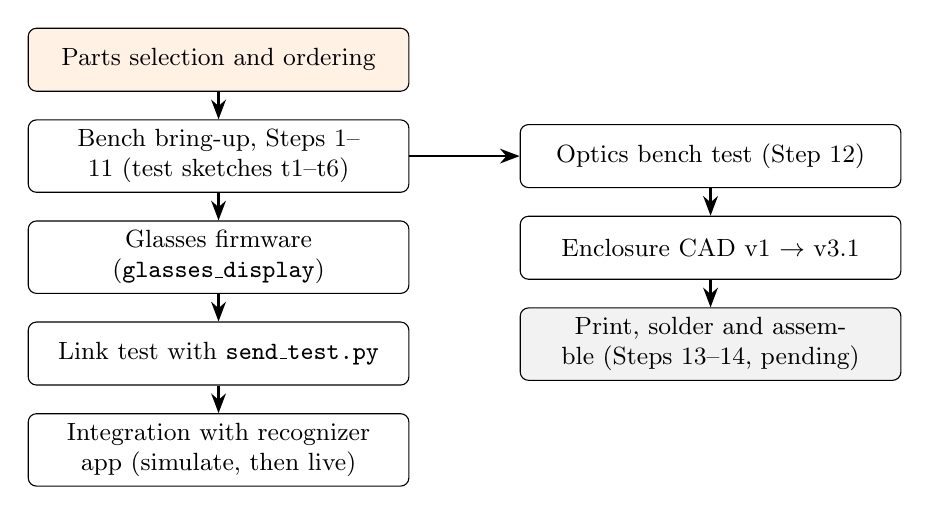
\begin{tikzpicture}[node distance=0.35cm]
  \node[flow,fill=orange!10] (a) {Parts selection and ordering};
  \node[flow,below=of a] (b) {Bench bring-up, Steps 1--11 (test sketches t1--t6)};
  \node[flow,below=of b] (c) {Glasses firmware (\texttt{glasses\_display})};
  \node[flow,below=of c] (d) {Link test with \texttt{send\_test.py}};
  \node[flow,below=of d] (e) {Integration with recognizer app (simulate, then live)};
  \node[flow,right=1.4cm of b] (f) {Optics bench test (Step 12)};
  \node[flow,below=of f] (g) {Enclosure CAD v1 $\rightarrow$ v3.1};
  \node[flow,below=of g,fill=gray!10] (h) {Print, solder and assemble (Steps 13--14, pending)};
  \draw[arr] (a)--(b); \draw[arr] (b)--(c); \draw[arr] (c)--(d); \draw[arr] (d)--(e);
  \draw[arr] (b)--(f); \draw[arr] (f)--(g); \draw[arr] (g)--(h);
\end{tikzpicture}
\caption{Design methodology and implementation flow}
\label{fig:workflow}
\end{figure}

\section{Hardware and Software Tools}

\begin{table}[H]
\centering
\caption{Hardware used for the display unit}
\label{tab:hw}
\begin{tabularx}{\linewidth}{L{5.2cm} c X}
\toprule
\textbf{Part} & \textbf{Qty} & \textbf{Purpose / note} \\
\midrule
ESP32-C3 SuperMini & 1 (+1) & Wi-Fi microcontroller, native USB-C \\
0.96'' SSD1306 OLED, 128$\times$64, I2C & 1 (+1) & Display, address 0x3C \\
LiPo 3.7 V, 600 mAh (602030) & 1 & Battery, $\sim$30$\times$20$\times$6 mm \\
TP4056 Type-C board with protection & 1 & Charger + over-discharge protection \\
Slide switch & 1 & Power on/off \\
25 mm lens (marked f45) & 1 & Magnifies the OLED image \\
Clear acrylic, 1 mm, 30$\times$30 mm & 1 & 45$^\circ$ beam combiner \\
PLA filament ($\sim$73 g) & -- & 3D-printed enclosure \\
Breadboard, berg strips, jumpers & -- & Bench bring-up \\
Bench supply, Rigol DM3058E meter & -- & Charging and measurements \\
\bottomrule
\end{tabularx}
\end{table}

\begin{table}[H]
\centering
\caption{Software and tools used}
\label{tab:sw}
\begin{tabularx}{\linewidth}{L{5.2cm} X}
\toprule
\textbf{Tool} & \textbf{Use} \\
\midrule
Arduino IDE 2.3, ESP32 core 3.3.12 & Firmware build and upload \\
Adafruit SSD1306 + GFX, WiFiUdp, ESPmDNS & OLED drawing, UDP, mDNS \\
Python, PyTorch, MediaPipe, OpenCV & Sign-recognition application \\
Python 3 + PyYAML & \texttt{send\_test.py} link-test tool \\
OpenSCAD & Parametric 3D enclosure, STL export \\
Git & Version control and daily work log \\
\bottomrule
\end{tabularx}
\end{table}

\section{Electronics and Wiring}
\begin{itemize}
  \item LiPo $\rightarrow$ TP4056 (B+/B$-$) $\rightarrow$ OUT+ $\rightarrow$ slide switch $\rightarrow$ ESP32-C3 \texttt{5V}; OUT$-$ $\rightarrow$ \texttt{G}.
  \item ESP32-C3 $\rightarrow$ OLED: \texttt{3V3}$\rightarrow$VDD, \texttt{G}$\rightarrow$GND, \texttt{GPIO8}$\rightarrow$SDA, \texttt{GPIO9}$\rightarrow$SCK (SCL).
  \item The ESP32-C3's on-board regulator gives 3.3\,V from the 3.7--4.2\,V cell.
  \item \textbf{Safety:} the TP4056 USB port is taped (``NO USB''); the cell is charged only from the bench supply.
\end{itemize}

\begin{figure}[H]
\centering
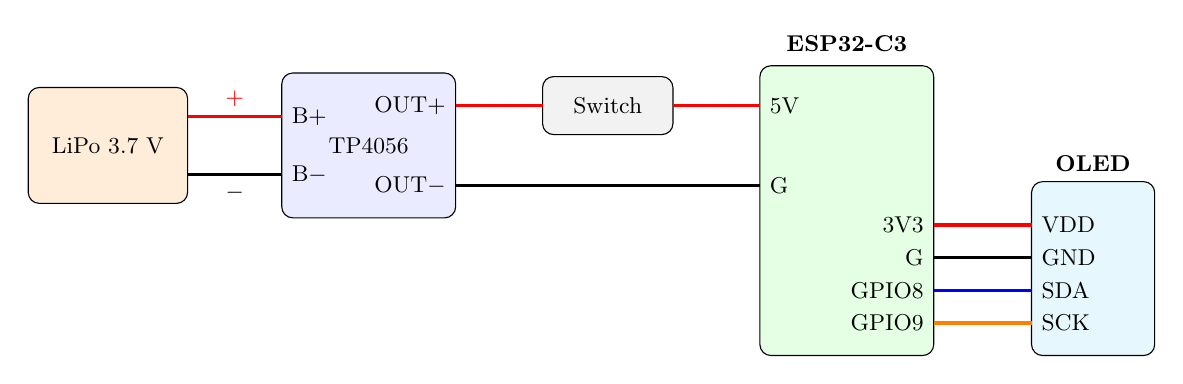
\begin{tikzpicture}[font=\small,scale=0.92,transform shape]
  \node[draw,rounded corners,fill=orange!15,minimum width=2.2cm,minimum height=1.6cm] (bat) at (0,0) {LiPo 3.7 V};
  \node[draw,rounded corners,fill=blue!8,minimum width=2.4cm,minimum height=2.0cm] (tp) at (3.6,0) {TP4056};
  \node[draw,rounded corners,fill=gray!10,minimum width=1.8cm,minimum height=0.8cm] (sw) at (6.9,0.55) {Switch};
  \node[draw,rounded corners,fill=green!10,minimum width=2.4cm,minimum height=4.0cm] (esp) at (10.2,-0.9) {};
  \node at (10.2,1.4) {\textbf{ESP32-C3}};
  \node[draw,rounded corners,fill=cyan!10,minimum width=1.7cm,minimum height=2.4cm] (ol) at (13.6,-1.7) {};
  \node at (13.6,-0.25) {\textbf{OLED}};
  \draw[red,very thick] (1.1,0.4) -- node[above]{+} (2.4,0.4) node[right,black]{B+};
  \draw[very thick] (1.1,-0.4) -- node[below]{$-$} (2.4,-0.4) node[right]{B$-$};
  \draw[red,very thick] (4.8,0.55) node[left,black]{OUT+} -- (6.0,0.55);
  \draw[red,very thick] (7.8,0.55) -- (9.0,0.55) node[right,black]{5V};
  \draw[very thick] (4.8,-0.55) node[left]{OUT$-$} -- (9.0,-0.55) node[right]{G};
  \foreach \y/\a/\b/\c in {-1.1/3V3/VDD/red, -1.55/G/GND/black, -2.0/GPIO8/SDA/blue, -2.45/GPIO9/SCK/orange}{
    \draw[\c,very thick] (11.4,\y) node[left,black]{\a} -- (12.75,\y) node[right,black]{\b};
  }
\end{tikzpicture}
\caption{Wiring of the glasses display unit}
\label{fig:wiring}
\end{figure}

\section{Firmware Design}
\begin{itemize}
  \item \textbf{Boot:} start I2C and the OLED, apply \texttt{MIRROR\_X}/\texttt{FLIP\_Y}, show \texttt{WIFI...}.
  \item \textbf{Network:} join the hotspot, lower Wi-Fi TX power to 8.5\,dBm (the SuperMini antenna is weak), start mDNS \texttt{glasses} and UDP port 4210, show \texttt{READY} + IP.
  \item \textbf{Receive:} read one datagram into a 256-byte buffer and pull the \texttt{"text"} value out of the JSON (a non-JSON packet is shown raw).
  \item \textbf{Display rule:} text at size 2 (12$\times$16 px per character) that fits 128\,px ($\le$10 characters) is centred; longer text scrolls right-to-left, 2 passes at 60\,px/s, then the screen goes blank.
  \item Scroll position is computed from elapsed time, so the speed stays constant however long a redraw takes.
\end{itemize}

\begin{figure}[H]
\centering
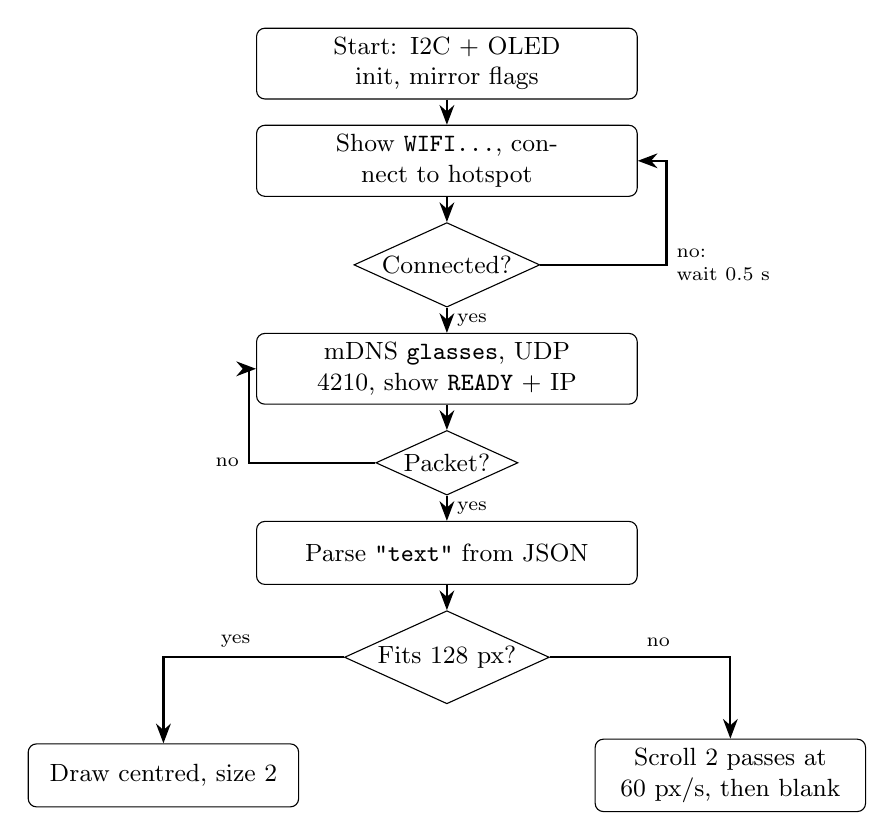
\begin{tikzpicture}[node distance=0.32cm]
  \node[flow] (s1) {Start: I2C + OLED init, mirror flags};
  \node[flow,below=of s1] (s2) {Show \texttt{WIFI...}, connect to hotspot};
  \node[dec,below=of s2] (d1) {Connected?};
  \node[flow,below=of d1] (s3) {mDNS \texttt{glasses}, UDP 4210, show \texttt{READY} + IP};
  \node[dec,below=of s3] (d2) {Packet?};
  \node[flow,below=of d2] (s4) {Parse \texttt{"text"} from JSON};
  \node[dec,below=of s4] (d3) {Fits 128 px?};
  \node[flow,text width=3.2cm] (s5) at ($(d3)+(-3.6,-1.5)$) {Draw centred, size 2};
  \node[flow,text width=3.2cm] (s6) at ($(d3)+(3.6,-1.5)$) {Scroll 2 passes at 60 px/s, then blank};
  \draw[arr] (s1)--(s2); \draw[arr] (s2)--(d1);
  \draw[arr] (d1)--node[right,font=\scriptsize]{yes}(s3);
  \draw[arr] (d1.east) -- ++(1.6,0) node[right,font=\scriptsize,align=left]{no:\\wait 0.5 s} |- (s2.east);
  \draw[arr] (s3)--(d2); \draw[arr] (d2)--node[right,font=\scriptsize]{yes}(s4);
  \draw[arr] (d2.west) -- ++(-1.6,0) node[left,font=\scriptsize]{no} |- (s3.west);
  \draw[arr] (s4)--(d3);
  \draw[arr] (d3.west) -| node[above,pos=0.3,font=\scriptsize]{yes} (s5.north);
  \draw[arr] (d3.east) -| node[above,pos=0.3,font=\scriptsize]{no} (s6.north);
\end{tikzpicture}
\caption{Firmware flowchart of the glasses receiver}
\label{fig:fwflow}
\end{figure}

\section{Optics Design}
\begin{itemize}
  \item The first design used a mirror and $u = 40$\,mm, based on the lens marking $f = 45$\,mm.
  \item The bench test (Step 12) showed a sharp image at only $u = 22$\,mm, so the mirror was removed.
  \item Final path: OLED (screen down) $\rightarrow$ 22\,mm $\rightarrow$ lens $\rightarrow$ 25\,mm $\rightarrow$ 45$^\circ$ acrylic $\rightarrow$ eye (Figure~\ref{fig:optics}).
  \item The OLED sits in rail slots at $u$ = 19, 22 or 25\,mm, so focus can be adjusted after printing.
\end{itemize}

\section{Enclosure Design}
\begin{itemize}
  \item Fully parametric (OpenSCAD, v3.1): optics distances, clearances, board sizes and glasses-arm sizes are named values.
  \item A pocket for each part (LiPo, TP4056, ESP32-C3, switch); the lid clicks shut and its fingers hold the boards.
  \item Clip-on mount: a dovetail slot in the body plus a swappable clip for the 7$\times$7\,mm temple arm.
  \item The build script stops with an error if any parts collide; the clip snap strain is checked (2.2\%, below PLA's $\sim$2.5\% limit).
\end{itemize}

\begin{figure}[H]
\centering
\begin{subfigure}{0.49\linewidth}\centering
  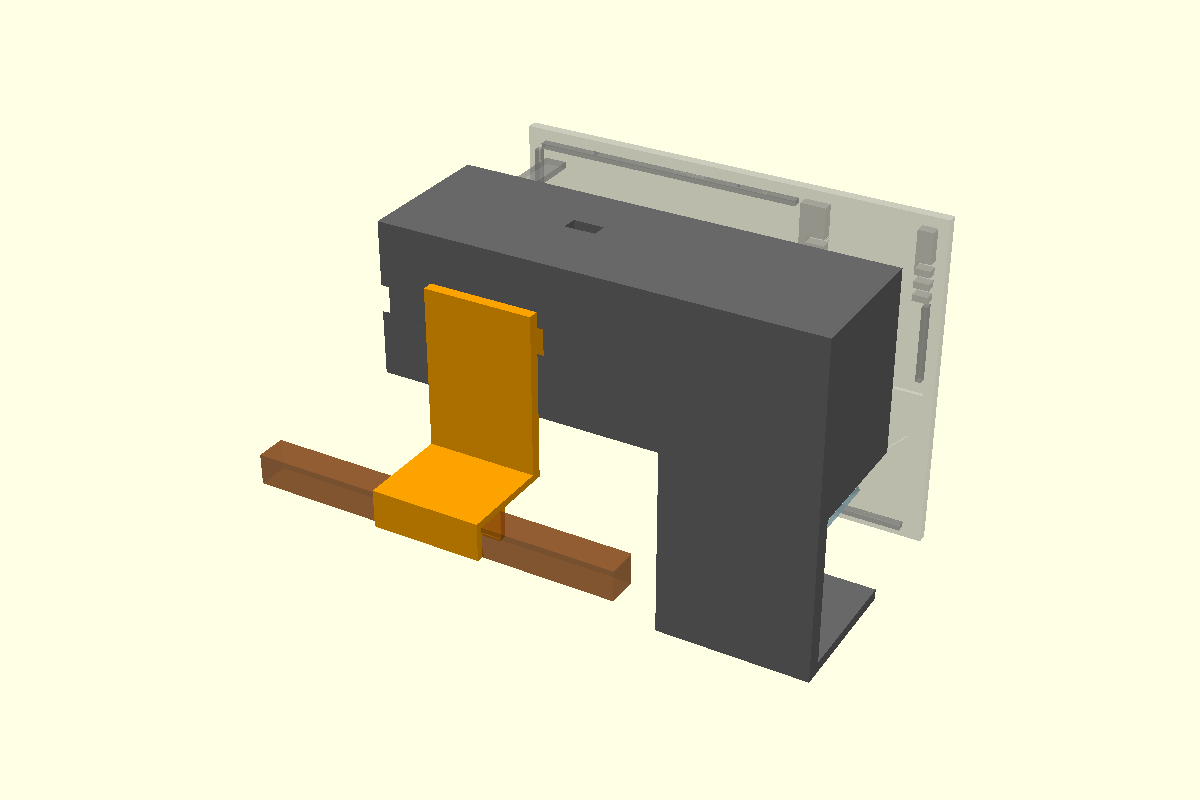
\includegraphics[width=\linewidth]{assembly.png}
  \caption{Assembly on the glasses arm (temple side)}
\end{subfigure}\hfill
\begin{subfigure}{0.49\linewidth}\centering
  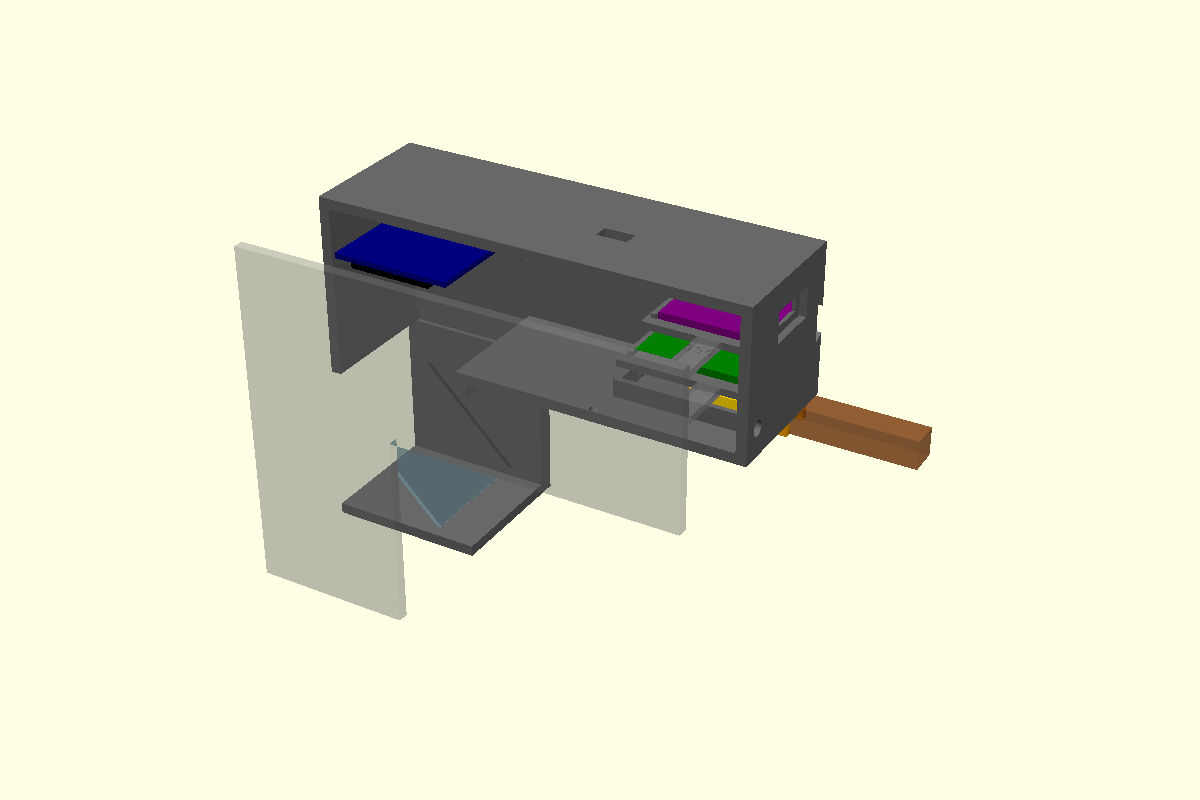
\includegraphics[width=\linewidth]{assembly_eye_side.png}
  \caption{Inside view (lid see-through)}
\end{subfigure}
\caption{3D model of the HUD display unit (OpenSCAD render)}
\label{fig:assembly}
\end{figure}

\begin{figure}[H]
\centering
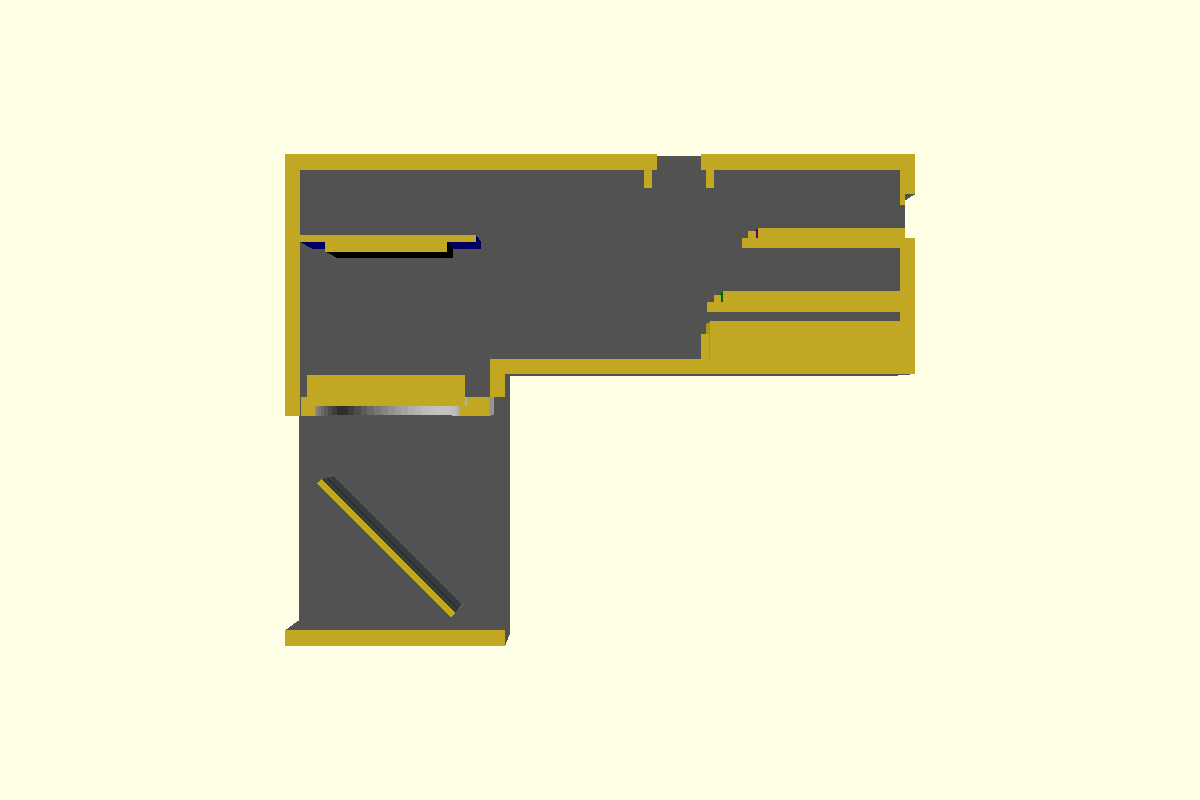
\includegraphics[width=0.6\linewidth]{section.png}
\caption{Cross-section of the enclosure: OLED rails at the top, lens plate, 45$^\circ$ acrylic in the head}
\label{fig:section}
\end{figure}

\section{Sign-Recognition Software}
\begin{itemize}
  \item Webcam $\rightarrow$ MediaPipe hand + body landmarks \cite{mediapipe} $\rightarrow$ TCN classifier \cite{tcn} (BiLSTM and Transformer also available) $\rightarrow$ sentence builder $\rightarrow$ optional English translation.
  \item Trained on INCLUDE-50 \cite{include} and our own recorded signs; runs on the laptop GPU.
  \item \texttt{glasses.py} sends each word, then the finished sentence, to the glasses over UDP \cite{sib}.
  \item A \texttt{--simulate} mode sends example sentences, so the glasses can be tested without a camera or model.
\end{itemize}

\section{Integration and Test Procedure}
\label{sec:proc}
\begin{enumerate}
  \item \textbf{Step 1:} visual check; measure the board's 5V and 3V3 pins with the multimeter.
  \item \textbf{Steps 2--3:} board on friction-fit headers; \texttt{t1\_blink} (LED + Serial \texttt{alive N}).
  \item \textbf{Step 4:} \texttt{t2\_i2c\_scan} (expect 0x3C), \texttt{t3\_oled\_hello}, mirror check.
  \item \textbf{Steps 5--6:} \texttt{t4\_wifi\_udp}; then on the laptop:\\ \texttt{python tools/send\_test.py --host <IP> --text hello}.
  \item \textbf{Steps 7--9:} TP4056 and switch on USB only; bench-charge the LiPo; solder the battery leads.
  \item \textbf{Steps 10--11:} run the ESP32-C3 from the battery; repeat the tests on the spare boards.
  \item \textbf{Step 12:} optics bench: slide the OLED until the text through the lens is sharpest; add the acrylic at 45$^\circ$.
  \item \textbf{Integration:} flash \texttt{glasses\_display}; run \texttt{python software/run.py --simulate}, then the live camera.
\end{enumerate}

\textbf{Packet format} (one UDP datagram per word or sentence, UTF-8 JSON, under 256 bytes):
\begin{lstlisting}[numbers=none]
{"text": "hello", "conf": 0.92}
\end{lstlisting}

\section{Phase-wise Work Summary}

\begin{table}[H]
\centering
\caption{Phase-wise work summary}
\label{tab:phases}
\begin{tabularx}{\linewidth}{L{2.6cm} X}
\toprule
\textbf{Date} & \textbf{Work done} \\
\midrule
24 Oct 2026 & Parts received; bring-up guide and test sketches written; Step 1 passed on both boards \\
25 Oct 2026 & Steps 3--6: blink, I2C scan (0x3C), OLED text, Wi-Fi + UDP text from the laptop \\
29 Oct 2026 & Enclosure v1 in OpenSCAD; LiPo checked; ESP32-C3 + OLED running on the battery \\
30 Oct 2026 & Enclosure v2: component pockets, click lid, dovetail clip mount \\
31 Oct 2026 & Steps 7--11 done; optics bench (sharp at 22 mm); enclosure v3/v3.1 print-ready; UDP interface written \\
1 Nov 2026 & Final receiver firmware; recognizer integrated with the glasses; simulated and live runs; documentation \\
\bottomrule
\end{tabularx}
\end{table}

% ═══════════════════════════════════════════════════════════════
%  CHAPTER 4: RESULTS AND DISCUSSION
% ═══════════════════════════════════════════════════════════════
\chapter{RESULTS AND DISCUSSION}

\section{Hardware Bring-Up Results}
\begin{itemize}
  \item All bring-up tests, Steps 1--11, passed on both sets of boards (Table~\ref{tab:bringup}).
  \item Typed text from the laptop appears on the OLED within about 0.5\,s (by eye), by IP address and by \texttt{glasses.local}.
  \item The whole chain works: simulated and live signing in front of the camera show words, then the sentence, on the OLED.
  \item Final firmware compiles to 79\% of the ESP32-C3 flash.
\end{itemize}

\begin{table}[H]
\centering
\caption{Hardware bring-up test results}
\label{tab:bringup}
\begin{tabularx}{\linewidth}{L{3.4cm} X c}
\toprule
\textbf{Part} & \textbf{Test} & \textbf{Result} \\
\midrule
ESP32-C3 \#1, \#2 & 5V/3V3 voltages, blink + Serial & Pass \\
OLED \#1, \#2 & I2C 0x3C, text, mirror view & Pass \\
Wi-Fi + UDP & \texttt{send\_test.py} text by IP and by \texttt{glasses.local} & Pass \\
TP4056 \#1, \#2 & B+ $\approx$ 4.2 V on USB (no cell) & Pass \\
Slide switch $\times$3 & Continuity swaps when flipped & Pass \\
Bench supply & 4.20 V / 0.30 A set and checked with the meter & Pass \\
LiPo \#1, \#2 & Voltage, soldered leads, ``NO USB'' tape & Pass \\
Battery power & \texttt{READY} + words on battery, switch on/off & Pass \\
Battery life & Runtime on a full cell & Done (value not logged) \\
Optics & Sharp text through lens + acrylic & In progress \\
Soldering, enclosure & Final build & Pending \\
\bottomrule
\end{tabularx}
\end{table}

\section{Electrical Measurements}

\begin{table}[H]
\centering
\caption{Measured electrical values (Rigol DM3058E)}
\label{tab:meas}
\begin{tabular}{l c}
\toprule
\textbf{Quantity} & \textbf{Measured} \\
\midrule
ESP32-C3 5V pin (USB), $V_{5V}$ & 5.162 V \\
ESP32-C3 3V3 pin (USB), $V_{3V3}$ & 3.302 V \\
LiPo \#1 as received & 3.999 V ($\sim$80\%) \\
ESP32-C3 5V pin on battery, under load & 3.967 V \\
Best focus, OLED to lens ($u$) & 22 mm \\
\bottomrule
\end{tabular}
\end{table}

\begin{itemize}
  \item 5.162\,V and 3.302\,V are inside the expected 4.8--5.2\,V and 3.2--3.4\,V ranges.
  \item On battery the 5V pin reads the cell voltage (3.967\,V) while 3V3 stays regulated, so the board runs safely on one LiPo cell.
\end{itemize}

\section{Display Timing Analysis}
At text size 2 each character is 12\,px wide; one pass moves the text across its own width plus the 128\,px screen:
\begin{equation}
t_{\text{pass}} = \frac{12\,n + 128}{60}\ \text{s}, \qquad t_{\text{total}} = 2\,t_{\text{pass}}
\label{eq:scroll}
\end{equation}
where $n$ is the number of characters and 60\,px/s is \texttt{SCROLL\_PX\_PER\_S}.

\begin{itemize}
  \item For ``I am going to school.'' ($n = 21$): $2 \times (12 \cdot 21 + 128)/60 = 12.67$\,s; plus the 2\,s word gap of the simulator = 14.67\,s.
  \item The measured gap was \textbf{14.6\,s}, so the firmware and the app stay in step (Figure~\ref{fig:scroll}).
\end{itemize}

\begin{figure}[H]
\centering
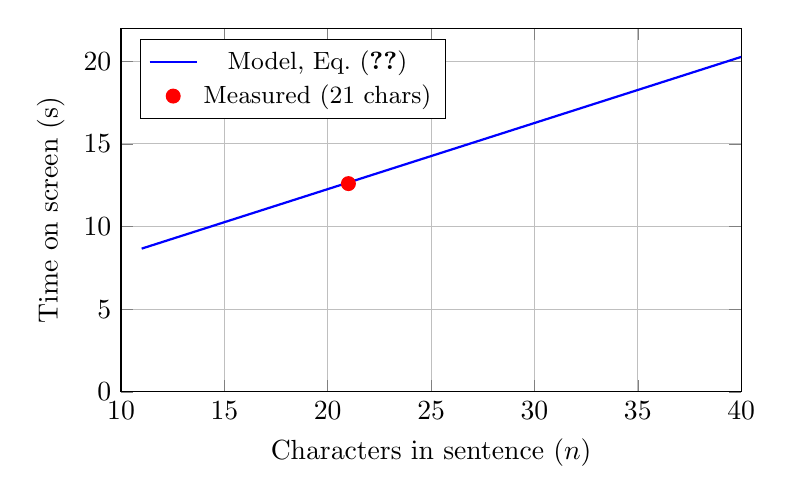
\begin{tikzpicture}
\begin{axis}[width=0.78\linewidth,height=6.2cm,xlabel={Characters in sentence ($n$)},ylabel={Time on screen (s)},
  xmin=10,xmax=40,ymin=0,ymax=22,grid=major,legend pos=north west,legend style={font=\small}]
  \addplot[thick,blue,domain=11:40,samples=2] {2*(12*x+128)/60};
  \addlegendentry{Model, Eq.~(\ref{eq:scroll})}
  \addplot[only marks,mark=*,red,mark size=2.5pt] coordinates {(21,12.6)};
  \addlegendentry{Measured (21 chars)}
\end{axis}
\end{tikzpicture}
\caption{Sentence scroll time vs.\ sentence length (2 passes at 60 px/s)}
\label{fig:scroll}
\end{figure}

\section{Optics Analysis}
With $u = 22$\,mm and an estimated $f \approx 25$\,mm, Eq.~(\ref{eq:lens}) gives
\[
\frac{1}{v} = \frac{1}{25} - \frac{1}{22} = \frac{22 - 25}{550} = -\frac{3}{550}
\;\Rightarrow\; v \approx -183~\text{mm}, \quad m = -\frac{v}{u} = \frac{183}{22} \approx 8.3
\]
\begin{itemize}
  \item The text appears as an upright, about 8$\times$ magnified virtual image roughly 18\,cm in front of the lens.
  \item The value of $f$ is an estimate; measuring it directly (Step 12, O5) is still pending.
\end{itemize}

\section{Enclosure Results}
\begin{itemize}
  \item Enclosure v3.1 is print-ready: all parts render with no collisions (Figures~\ref{fig:parts} and \ref{fig:bed}).
  \item All four parts fit on one print bed: about 73\,g of PLA (Table~\ref{tab:print}).
\end{itemize}

\begin{figure}[H]
\centering
\begin{subfigure}{0.32\linewidth}\centering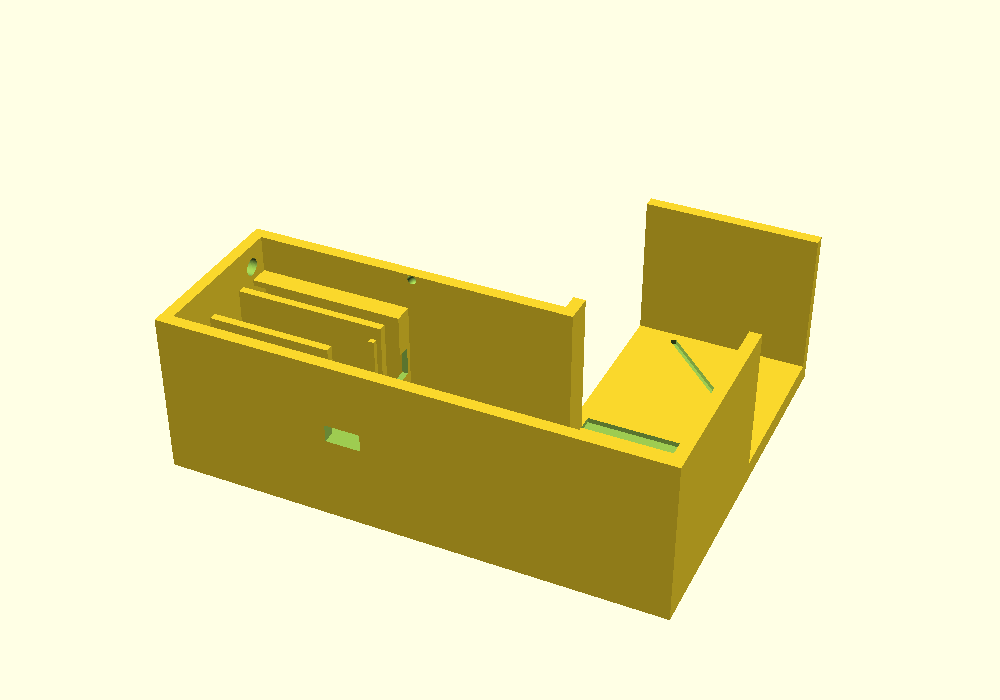
\includegraphics[width=\linewidth]{body.png}\caption{Body}\end{subfigure}\hfill
\begin{subfigure}{0.32\linewidth}\centering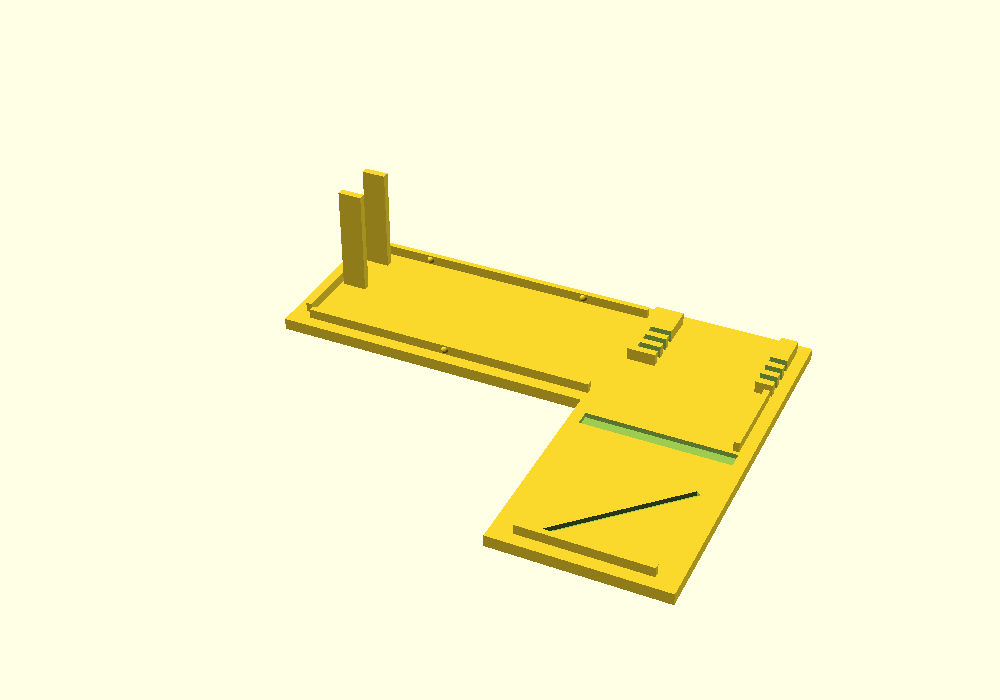
\includegraphics[width=\linewidth]{lid.png}\caption{Lid}\end{subfigure}\hfill
\begin{subfigure}{0.32\linewidth}\centering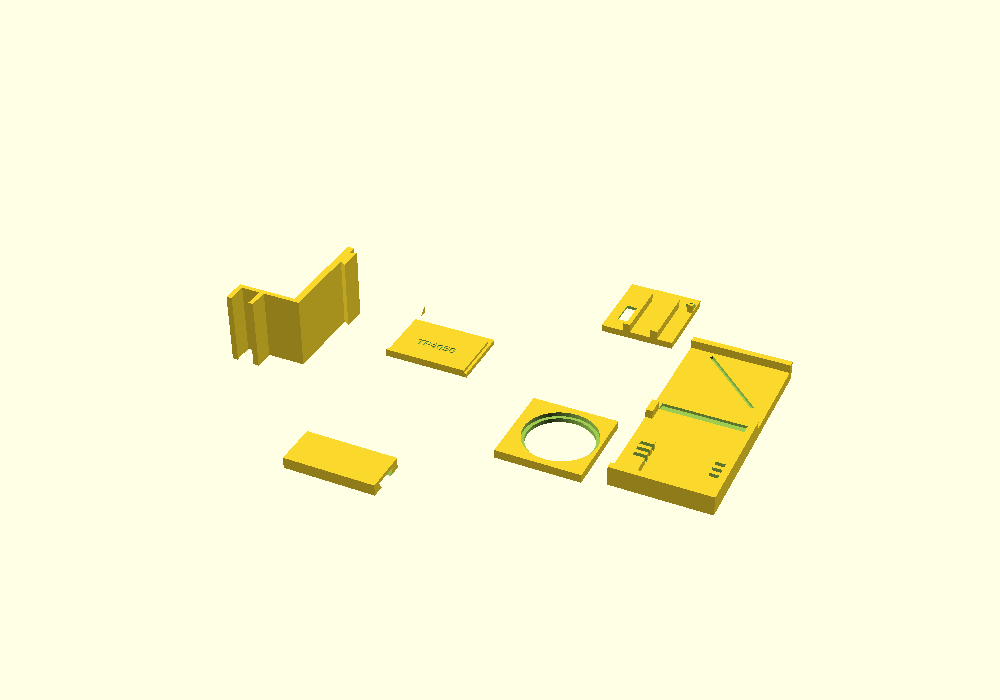
\includegraphics[width=\linewidth]{test_fit.png}\caption{Test-fit piece}\end{subfigure}\\[6pt]
\begin{subfigure}{0.32\linewidth}\centering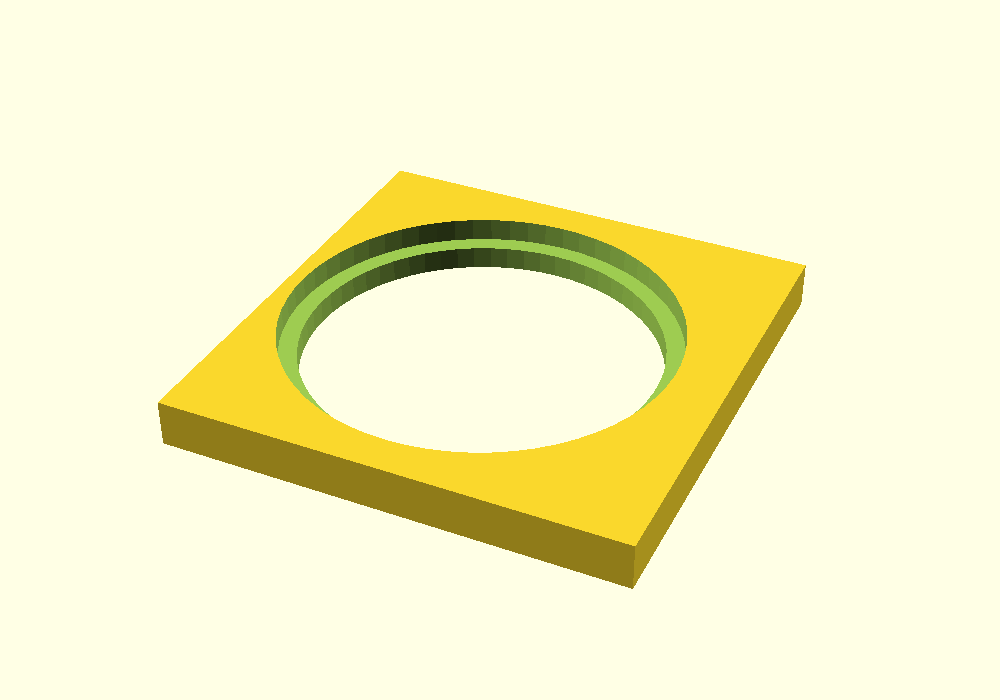
\includegraphics[width=\linewidth]{lens_plate.png}\caption{Lens plate}\end{subfigure}\hspace{0.02\linewidth}
\begin{subfigure}{0.32\linewidth}\centering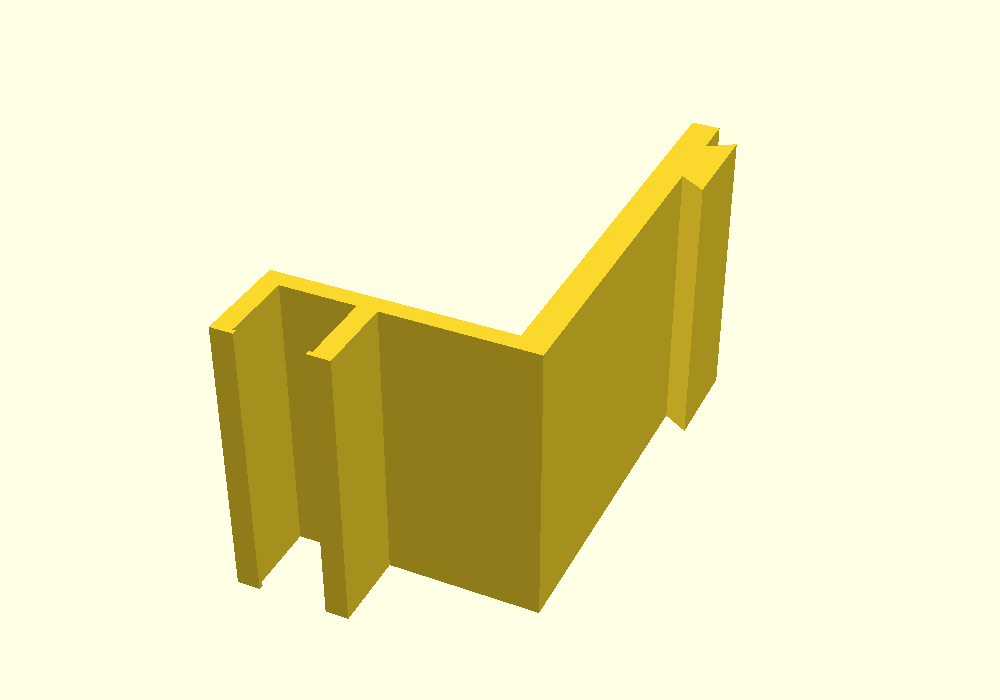
\includegraphics[width=\linewidth]{clip.png}\caption{Clip}\end{subfigure}
\caption{Printable enclosure parts (OpenSCAD renders)}
\label{fig:parts}
\end{figure}

\begin{figure}[H]
\centering
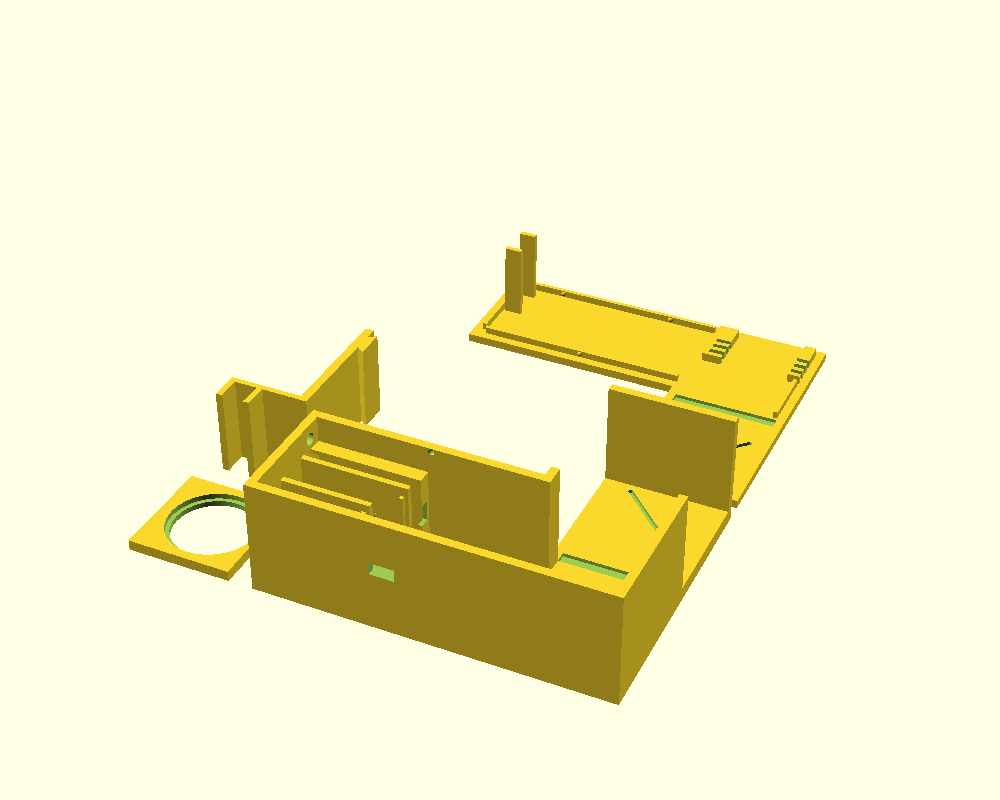
\includegraphics[width=0.55\linewidth]{print_all.png}
\caption{All four parts laid out on one print bed (137 $\times$ 161 mm)}
\label{fig:bed}
\end{figure}

\begin{table}[H]
\centering
\caption{Enclosure parts: plastic and print time (slicer estimates)}
\label{tab:print}
\begin{tabular}{l c c}
\toprule
\textbf{Part} & \textbf{PLA (g)} & \textbf{Time (normal / fast printer)} \\
\midrule
Body & 50 & 4.2 h / 1.7 h \\
Lid & 16 & 1.3 h / 0.5 h \\
Clip & 5 & 0.4 h / 0.2 h \\
Lens plate & 2 & 0.1 h \\
\textbf{All on one bed} & \textbf{$\sim$73} & \textbf{$\sim$6 h / $\sim$2.5 h} \\
Test-fit piece (optional) & 27 & 2.2 h / 0.9 h \\
\bottomrule
\end{tabular}
\end{table}

% PHOTO SLOTS: uncomment and add your photos in figures/ when available.
% \begin{figure}[H]\centering
% \includegraphics[width=0.7\linewidth]{photo_breadboard.jpg}
% \caption{Breadboard set-up: ESP32-C3 + OLED showing a received word}\label{fig:photo_bench}
% \end{figure}
% \begin{figure}[H]\centering
% \includegraphics[width=0.7\linewidth]{photo_glasses.jpg}
% \caption{Assembled HUD unit on the glasses}\label{fig:photo_glasses}
% \end{figure}

\section{Comparison with Expected Results}

\begin{table}[H]
\centering
\caption{Expected (design) vs.\ obtained results}
\label{tab:compare}
\begin{tabularx}{\linewidth}{L{3.4cm} X X}
\toprule
\textbf{Item} & \textbf{Expected} & \textbf{Obtained} \\
\midrule
Focus distance $u$ & 40 mm (lens marked $f = 45$ mm; Eq.~(\ref{eq:lens}) gives $v = -360$ mm, $m = 9$) & 22 mm; real $f$ $\approx$ 25 mm; mirror removed \\
Sentence time ($n = 21$) & 12.67 s scroll + 2 s gap = 14.67 s & 14.6 s measured \\
3V3 rail & 3.2--3.4 V & 3.302 V \\
5V rail on USB & 4.8--5.2 V & 5.162 V \\
I2C address & 0x3C & 0x3C on both OLEDs \\
mDNS discovery & \texttt{glasses.local} resolves & Works; sometimes slow, IP fallback used \\
Clip snap strain & below PLA limit ($\sim$2.5\%) & 2.2\% (model check) \\
\bottomrule
\end{tabularx}
\end{table}

\section{Challenges and Solutions}

\subsection{Technical Challenges}
\begin{itemize}
  \item The lens did not behave like its marking ($f = 45$\,mm): the image was sharp at 22\,mm, not 40\,mm.
  \item The ESP32-C3 SuperMini often failed to connect at full Wi-Fi transmit power.
  \item The ESP32-C3 cannot join 5\,GHz hotspots.
  \item \texttt{glasses.local} (mDNS) was sometimes not found from the laptop.
  \item A 4-line word-wrap made sentences cramped and hard to read on a 128$\times$64 screen.
  \item The simulator first sent ISL glosses (``TODAY HOT''), so words like ``is'' never appeared.
\end{itemize}

\subsection{Practical Challenges}
\begin{itemize}
  \item The stock TP4056 charges at 1\,A, which is too high for a 600\,mAh cell.
  \item Arduino's build tool (\texttt{ctags}) is x86-only and failed on the Apple Silicon laptop (``bad CPU type in executable'').
  \item Port 8000 on the laptop was already in use by another application.
  \item Loose friction-fit headers gave random resets and ``no I2C device'' errors.
  \item Board and lens sizes were not all measured before the enclosure design.
\end{itemize}

\begin{table}[H]
\centering
\caption{Problems and the actions taken}
\label{tab:solutions}
\begin{tabularx}{\linewidth}{L{5cm} X}
\toprule
\textbf{Problem} & \textbf{Action taken} \\
\midrule
Lens focus at 22 mm, not 40 mm & Mirror removed; OLED rails at 19/22/25 mm; enclosure v3 \\
Wi-Fi fails at full TX power & \texttt{WiFi.setTxPower(WIFI\_POWER\_8\_5dBm)} \\
5 GHz hotspot & 2.4 GHz hotspot (``Maximize Compatibility'' on iPhone) \\
mDNS not always found & IP shown on the OLED; \texttt{--glasses <IP>} / \texttt{--host <IP>} option \\
Cramped sentences & One-line, right-to-left scroll, 2 passes, then blank \\
Simulator showed glosses & Simulator sends the English sentence word by word \\
1 A charge current & USB port taped; bench supply 4.20 V / 0.30 A, stop at $\le$ 0.05 A \\
\texttt{ctags} ``bad CPU type'' & Installed Rosetta 2 \\
Port 8000 busy & App started with \texttt{--port 9000} \\
Loose headers & Press the board down first; solder only in the final build \\
Unmeasured part sizes & 0.3 mm pocket clearance; print the test-fit piece first \\
\bottomrule
\end{tabularx}
\end{table}

% ═══════════════════════════════════════════════════════════════
%  CHAPTER 5: CONCLUSION AND FUTURE WORK
% ═══════════════════════════════════════════════════════════════
\chapter{CONCLUSION AND FUTURE WORK}

\section{Conclusion}
\begin{itemize}
  \item A working, low-cost chain from an ISL signer to text in a wearable HUD was built and tested.
  \item All hardware bring-up tests (Steps 1--11) passed.
  \item The display firmware finds the laptop by name, centres short words and scrolls sentences.
  \item The end-to-end demo works: camera $\rightarrow$ recognizer $\rightarrow$ Wi-Fi $\rightarrow$ glasses.
  \item The parametric clip-on enclosure is print-ready ($\sim$73\,g PLA).
  \item Measured values match the design model, e.g.\ sentence timing within 0.1\,s.
\end{itemize}

\section{Limitations and Assumptions}
\begin{itemize}
  \item The lens focal length ($f \approx 25$\,mm) is estimated from the focus distance, not measured.
  \item Glasses-side latency, end-to-end delay and recognition accuracy have not been measured yet.
  \item Battery runtime was tested but the value was not logged.
  \item The enclosure is designed and exported but not yet printed or assembled.
  \item The firmware has no ``NO LINK'' screen and no automatic Wi-Fi reconnect yet.
  \item The system needs a laptop and a 2.4\,GHz phone hotspot; it recognises isolated words, not continuous signing.
\end{itemize}

\section{Future Work}
\begin{itemize}
  \item Show ``NO LINK'' after 10\,s without packets, and reconnect to Wi-Fi automatically.
  \item Measure the glasses-side latency (packet in $\rightarrow$ OLED update) and the end-to-end delay.
  \item Measure the lens focal length directly (Step 12, O5), and check readability in daylight.
  \item Print, solder and assemble the final unit (Steps 13--14), and measure the battery runtime.
  \item Report the recognition accuracy of the model on a held-out test set.
  \item Add the ESP32-CAM on the glasses as the camera, so the laptop camera is not needed.
\end{itemize}

% ═══════════════════════════════════════════════════════════════
%  REFERENCES
% ═══════════════════════════════════════════════════════════════
\clearpage
\phantomsection
\addcontentsline{toc}{chapter}{REFERENCES}
\begin{thebibliography}{99}
\raggedright
\bibitem{esp32c3} Espressif Systems, ``ESP32-C3 Series Datasheet,'' Espressif Systems, Shanghai, China. [Online]. Available: \url{https://www.espressif.com}
\bibitem{ssd1306} Solomon Systech, ``SSD1306: 128 x 64 Dot Matrix OLED/PLED Segment/Common Driver with Controller,'' datasheet, Rev.~1.1, 2008.
\bibitem{tp4056} NanJing Top Power ASIC Corp., ``TP4056: 1A Standalone Linear Li-ion Battery Charger with Thermal Regulation in SOP-8,'' datasheet.
\bibitem{mediapipe} C. Lugaresi \emph{et al.}, ``MediaPipe: A framework for building perception pipelines,'' arXiv:1906.08172, 2019.
\bibitem{include} A. Sridhar, R. G. Ganesan, P. Kumar, and M. Khapra, ``INCLUDE: A large scale dataset for Indian Sign Language recognition,'' in \emph{Proc. 28th ACM Int. Conf. Multimedia}, 2020, pp.~1366--1375.
\bibitem{tcn} S. Bai, J. Z. Kolter, and V. Koltun, ``An empirical evaluation of generic convolutional and recurrent networks for sequence modeling,'' arXiv:1803.01271, 2018.
\bibitem{hecht} E. Hecht, \emph{Optics}, 5th ed. Boston, MA, USA: Pearson, 2017.
\bibitem{adafruit1306} Adafruit Industries, ``Adafruit\_SSD1306 Arduino library,'' GitHub. [Online]. Available: \url{https://github.com/adafruit/Adafruit_SSD1306}
\bibitem{adafruitgfx} Adafruit Industries, ``Adafruit-GFX-Library,'' GitHub. [Online]. Available: \url{https://github.com/adafruit/Adafruit-GFX-Library}
\bibitem{openscad} OpenSCAD, ``OpenSCAD: The programmers solid 3D CAD modeller.'' [Online]. Available: \url{https://openscad.org}
\bibitem{june} perseus784, ``June\_Glasses,'' GitHub. [Online]. Available: \url{https://github.com/perseus784/June_Glasses}
\bibitem{sib} integral-830, ``sign-inference-bridge: ISL recognition application,'' GitHub. [Online]. Available: \url{https://github.com/integral-830/sign-inference-bridge}
\end{thebibliography}

% ═══════════════════════════════════════════════════════════════
%  APPENDICES
% ═══════════════════════════════════════════════════════════════
\appendix
\titleformat{\chapter}[display]{\normalfont\bfseries\centering\Large}{APPENDIX \thechapter}{0.5em}{\Large}

\chapter{WIRING AND BILL OF MATERIALS}

\section{Wiring Table}
\begin{table}[H]
\centering
\caption{Display unit wiring}
\label{tab:wiring}
\begin{tabular}{l l}
\toprule
\textbf{From} & \textbf{To} \\
\midrule
LiPo red / black & TP4056 B+ / B$-$ (soldered) \\
TP4056 OUT+ & Switch middle pin; switch side pin $\rightarrow$ ESP32-C3 5V \\
TP4056 OUT$-$ & ESP32-C3 G \\
ESP32-C3 3V3 & OLED VDD (VCC) \\
ESP32-C3 G & OLED GND \\
ESP32-C3 GPIO8 & OLED SDA \\
ESP32-C3 GPIO9 & OLED SCK (SCL) \\
\bottomrule
\end{tabular}
\end{table}

\section{Bill of Materials}
\begin{itemize}
  \item ESP32-C3 SuperMini $\times$2, 0.96'' SSD1306 OLED $\times$2, TP4056 Type-C board $\times$2, slide switch $\times$3.
  \item LiPo 3.7\,V 600\,mAh (602030) $\times$2, 25\,mm lens pair, 1\,mm clear acrylic $\times$4.
  \item Breadboard, berg strips, jumper wires, soldering kit with multimeter, Type-C cable.
  \item About 73\,g of black PLA for the enclosure.
\end{itemize}

\chapter{FIRMWARE SOURCE EXCERPT}
Main display functions of \texttt{firmware/glasses\_display/glasses\_display.ino}:
\begin{lstlisting}[language=C++]
// New text: fits on the screen -> static in the centre; wider -> start scrolling.
void showText(const String &text) {
  int16_t x1, y1;
  uint16_t w, h;
  display.setTextSize(2);
  display.getTextBounds(text, 0, 0, &x1, &y1, &w, &h);
  if (w <= display.width()) {
    scrollText = "";
    display.clearDisplay();
    drawCentered(text, 2, (display.height() - 16) / 2);
    display.display();
  } else {
    scrollText = text;
    scrollW = w;
    scrollStart = millis();
    lastFrame = 0;
  }
}

void loop() {
  int len = udp.parsePacket();
  if (len > 0) {
    len = udp.read(packet, sizeof(packet) - 1);
    packet[len] = '\0';
    showText(jsonText(String(packet)));
  }
  if (scrollText.length() && millis() - lastFrame >= FRAME_MS) {
    lastFrame = millis();
    scrollFrame();
  }
}
\end{lstlisting}

\chapter{UDP INTERFACE AND TEST TOOLS}
\begin{itemize}
  \item Glasses: mDNS name \texttt{glasses.local}, UDP port 4210 (from \texttt{config.yaml}).
  \item One datagram per word or sentence, UTF-8 JSON, under 256 bytes:
\end{itemize}
\begin{lstlisting}[numbers=none]
{"text": "hello", "conf": 0.92}
\end{lstlisting}
\begin{itemize}
  \item \texttt{text}: word or short line to show; \texttt{conf}: model confidence, 0--1, 2 decimals.
  \item Test without the recognizer: \texttt{python tools/send\_test.py --text hello}
  \item Simulated signing: \texttt{python software/run.py --simulate --port 9000}
  \item Source code: \url{https://github.com/Charan20510/sign_lang_hud_glasses}
\end{itemize}

\chapter{BRING-UP TEST SKETCHES}
\begin{itemize}
  \item \texttt{t1\_blink}: board alive (LED + Serial).
  \item \texttt{t2\_i2c\_scan}: finds the OLED at 0x3C.
  \item \texttt{t3\_oled\_hello}: big ``HELLO'' + counter.
  \item \texttt{t4\_wifi\_udp}: text from the laptop over Wi-Fi.
  \item \texttt{t5\_icons}: bitmap image on the OLED.
  \item \texttt{t6\_mirror\_center}: mirrored, centred text for the HUD view.
\end{itemize}
Full step-by-step guide: \texttt{docs/hardware\_bringup.md}; run guide: \texttt{docs/run\_guide.md}.

\end{document}
